% To je predloga za poročila o domačih nalogah pri predmetih, katerih
% nosilec je Blaž Zupan. Seveda lahko tudi dodaš kakšen nov, zanimiv
% in uporaben element, ki ga v tej predlogi (še) ni. Več o LaTeX-u izveš na
% spletu, na primer na http://tobi.oetiker.ch/lshort/lshort.pdf.
%
% To predlogo lahko spremeniš v PDF dokument s pomočjo programa
% pdflatex, ki je del standardne instalacije LaTeX programov.

\documentclass[a4paper,11pt]{article}
\usepackage{a4wide}
\usepackage{fullpage}
\usepackage[utf8x]{inputenc}
\usepackage[slovene]{babel}
\selectlanguage{slovene}
\usepackage[toc,page]{appendix}
\usepackage[pdftex]{graphicx} % za slike
\usepackage{setspace}
\usepackage{color}
\definecolor{light-gray}{gray}{0.95}
\usepackage{listings} % za vključevanje kode
\usepackage{hyperref}
\renewcommand{\baselinestretch}{1.2} % za boljšo berljivost večji razmak
\renewcommand{\appendixpagename}{Priloge}

\lstset{ % nastavitve za izpis kode, sem lahko tudi kaj dodaš/spremeniš
language=Python,
basicstyle=\footnotesize,
basicstyle=\ttfamily\footnotesize\setstretch{1},
backgroundcolor=\color{light-gray},
}

\title{Stiskanje in čiščenje slik s pomočjo DVT}
\author{David Rubin (david.rubin@student.um.si)}
\date{\today}

\begin{document}

\maketitle

\section{Uvod}

S pomočjo poljubne knjižnice izračunajte diskretno valčno transformacijo (DVT) slike. Izberite najprimernejši valček za vašo sliko. Število nivojev dekompozicije določite sami. Dobro preverite, kako so v izhodu DVT-ja zapisane podrobnosti in približki vhodne slike. 

Nad rezultatom DVT uporabite ali trdo ali mehko odstranjevanje motenj in visokih frekvenc, pri čemer testirajte različne pragovne vrednosti odstranjevanja. S pomočjo inverzne DVT spremenjene valčne koeficiente preslikajte nazaj v prostorsko domeno slik in jih primerjajte z originalno  sliko:
\begin{enumerate}
\item Testirajte vsaj štiri različne slike, ki naj bodo čimbolj različne. 
\item Vsaki sliki določite optimalni valček (testirajte vsaj tri različne valčke) in optimalen prag rezanja (testirajte vsaj štiri različne pragove rezanja). 
\item Ocenite stopnjo stiskanja in kvaliteto rekonstrukcije s pomočjo inverzne  DVT. Podobnosti oz. odstopanja med originalno in rekonstruirano sliko merite s korelacijskim koeficientom in normalizirano kvadratično napako (normalized root-mean-square deviation).
\item Za izbrane pragove rezanja ocenite razliko med mehkim in trdim pragovnim odstranjevanjem motenj. 
\item Postopke testiranja na izbrani sliki (lahko je ena sama) ponovite ob prisotnosti 20 dB belega šuma, ki ga tvorite sami.
\end{enumerate}

\section{Rezultati}

Za testiranje svoje rešitve sem si izbral 4 slike (slike~\ref{slika1}, ~\ref{slika2}, ~\ref{slika3} in ~\ref{slika4}). Testiral sem 7 različnih valčkov, ki so skupaj z grafi prikazani na sliki~\ref{wavelets}. Rešitev je implementirana kot Python program (\textit{dwt.py}), zahtevane knjižnice pa so naštete znotraj \textit{requirements.txt}.

Nad 7 omenjenih valčkov sem testiral kombinacije naslednjih parametrov
\begin{itemize}
	\item pragovi rezanja ... [2, 20, 50, 150],
    \item mehko in trdo pragovno odstranjevanje motenj,
    \item število nivojev dekompozicije ... [1, 4, 9],
\end{itemize}
kar skupaj nanese 96 kombinacij. Rezultati vsakega poskusa stiskanja (Pearsonova korelacija, normaliziran RMSE in kompresijsko razmerje) so shranjeni v direktoriju \textit{metrics/}, kjer je ime datoteke sestavljeno kot:
$$slika\_prag\_funkcija\_dekompozicija.csv$$
Datoteka je v .csv formatu, kjer prva vrstica predstavlja imena stolpcev (\textit{header)}, naslednjih 7 pa vsebuje prej omenjene metrike za vsak posamezen valček.

\begin{figure}[htbp]
\begin{center}
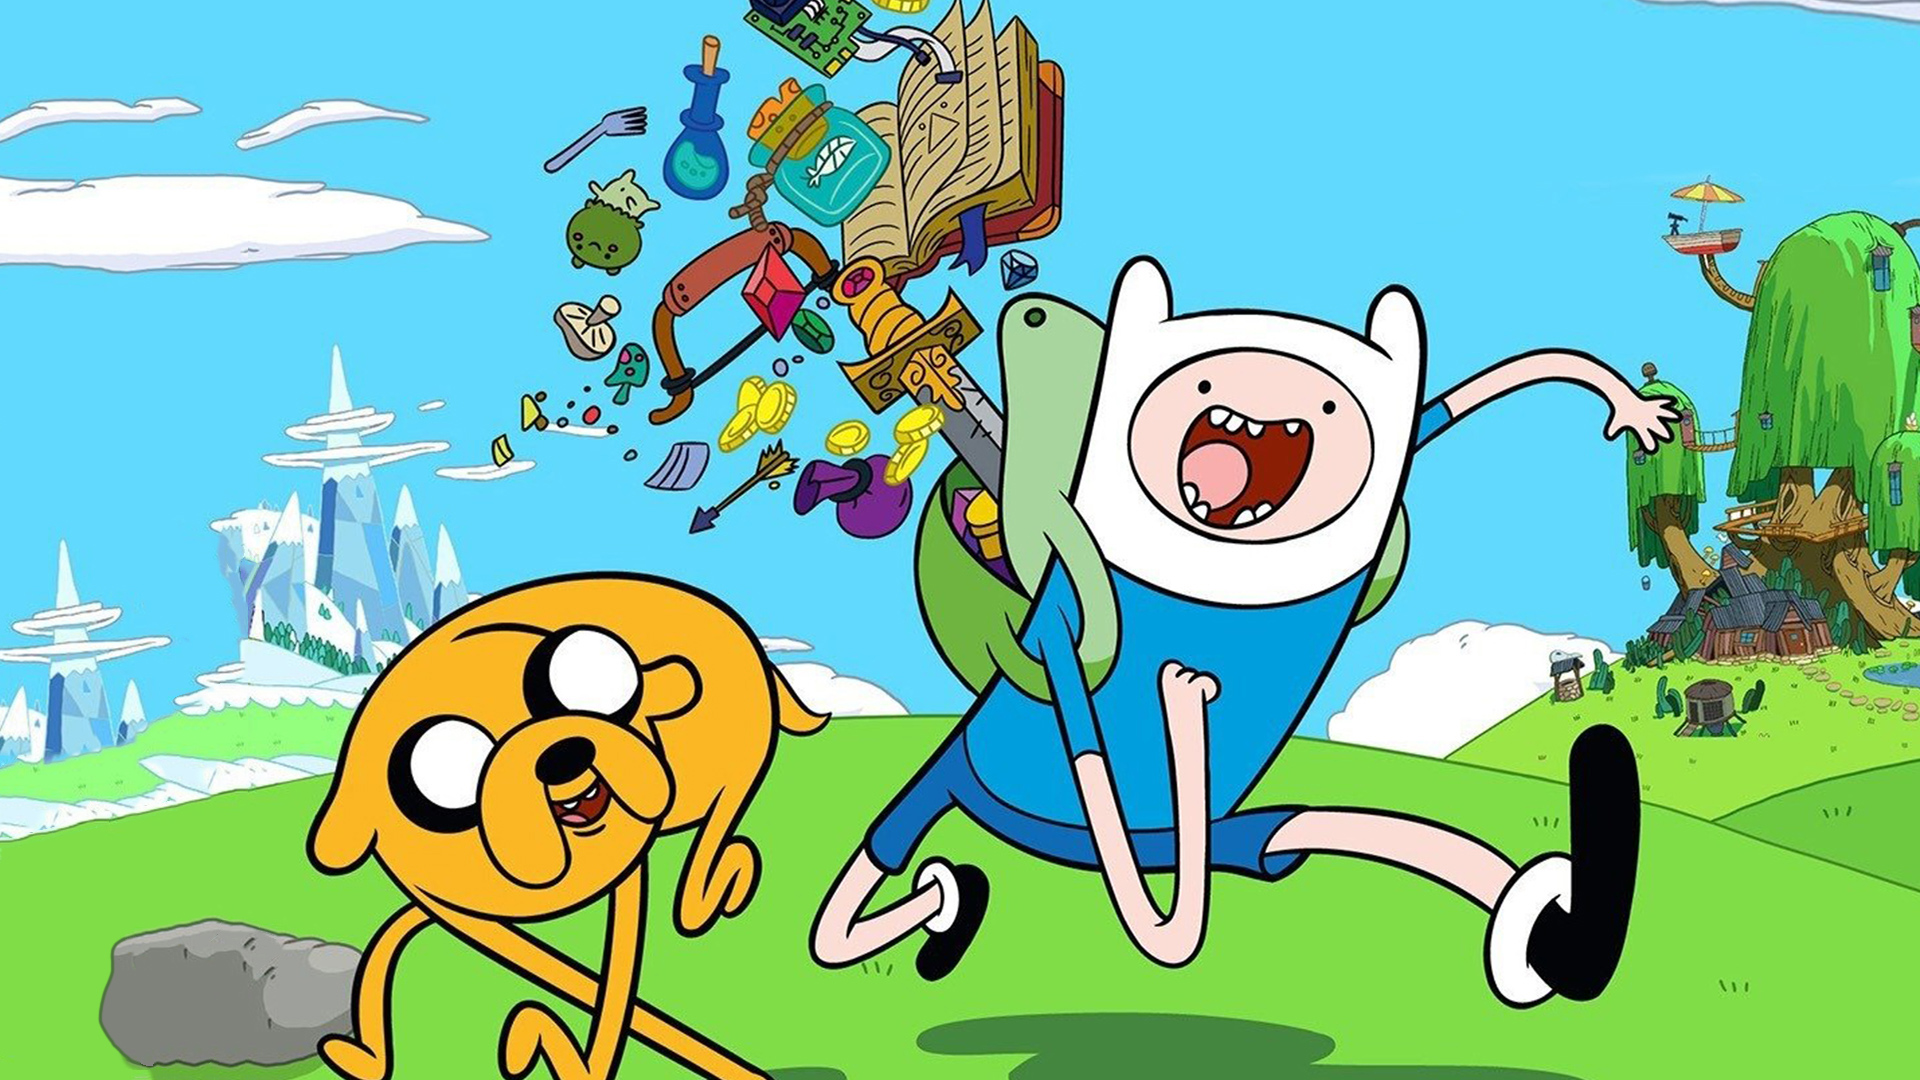
\includegraphics[width=1\textwidth]{images/adventuretime.jpg}
\caption{Slika iz risanke, veliko ostrih prehodov brav.}
\label{slika1}
\end{center}
\end{figure}

\begin{figure}[htbp]
\begin{center}
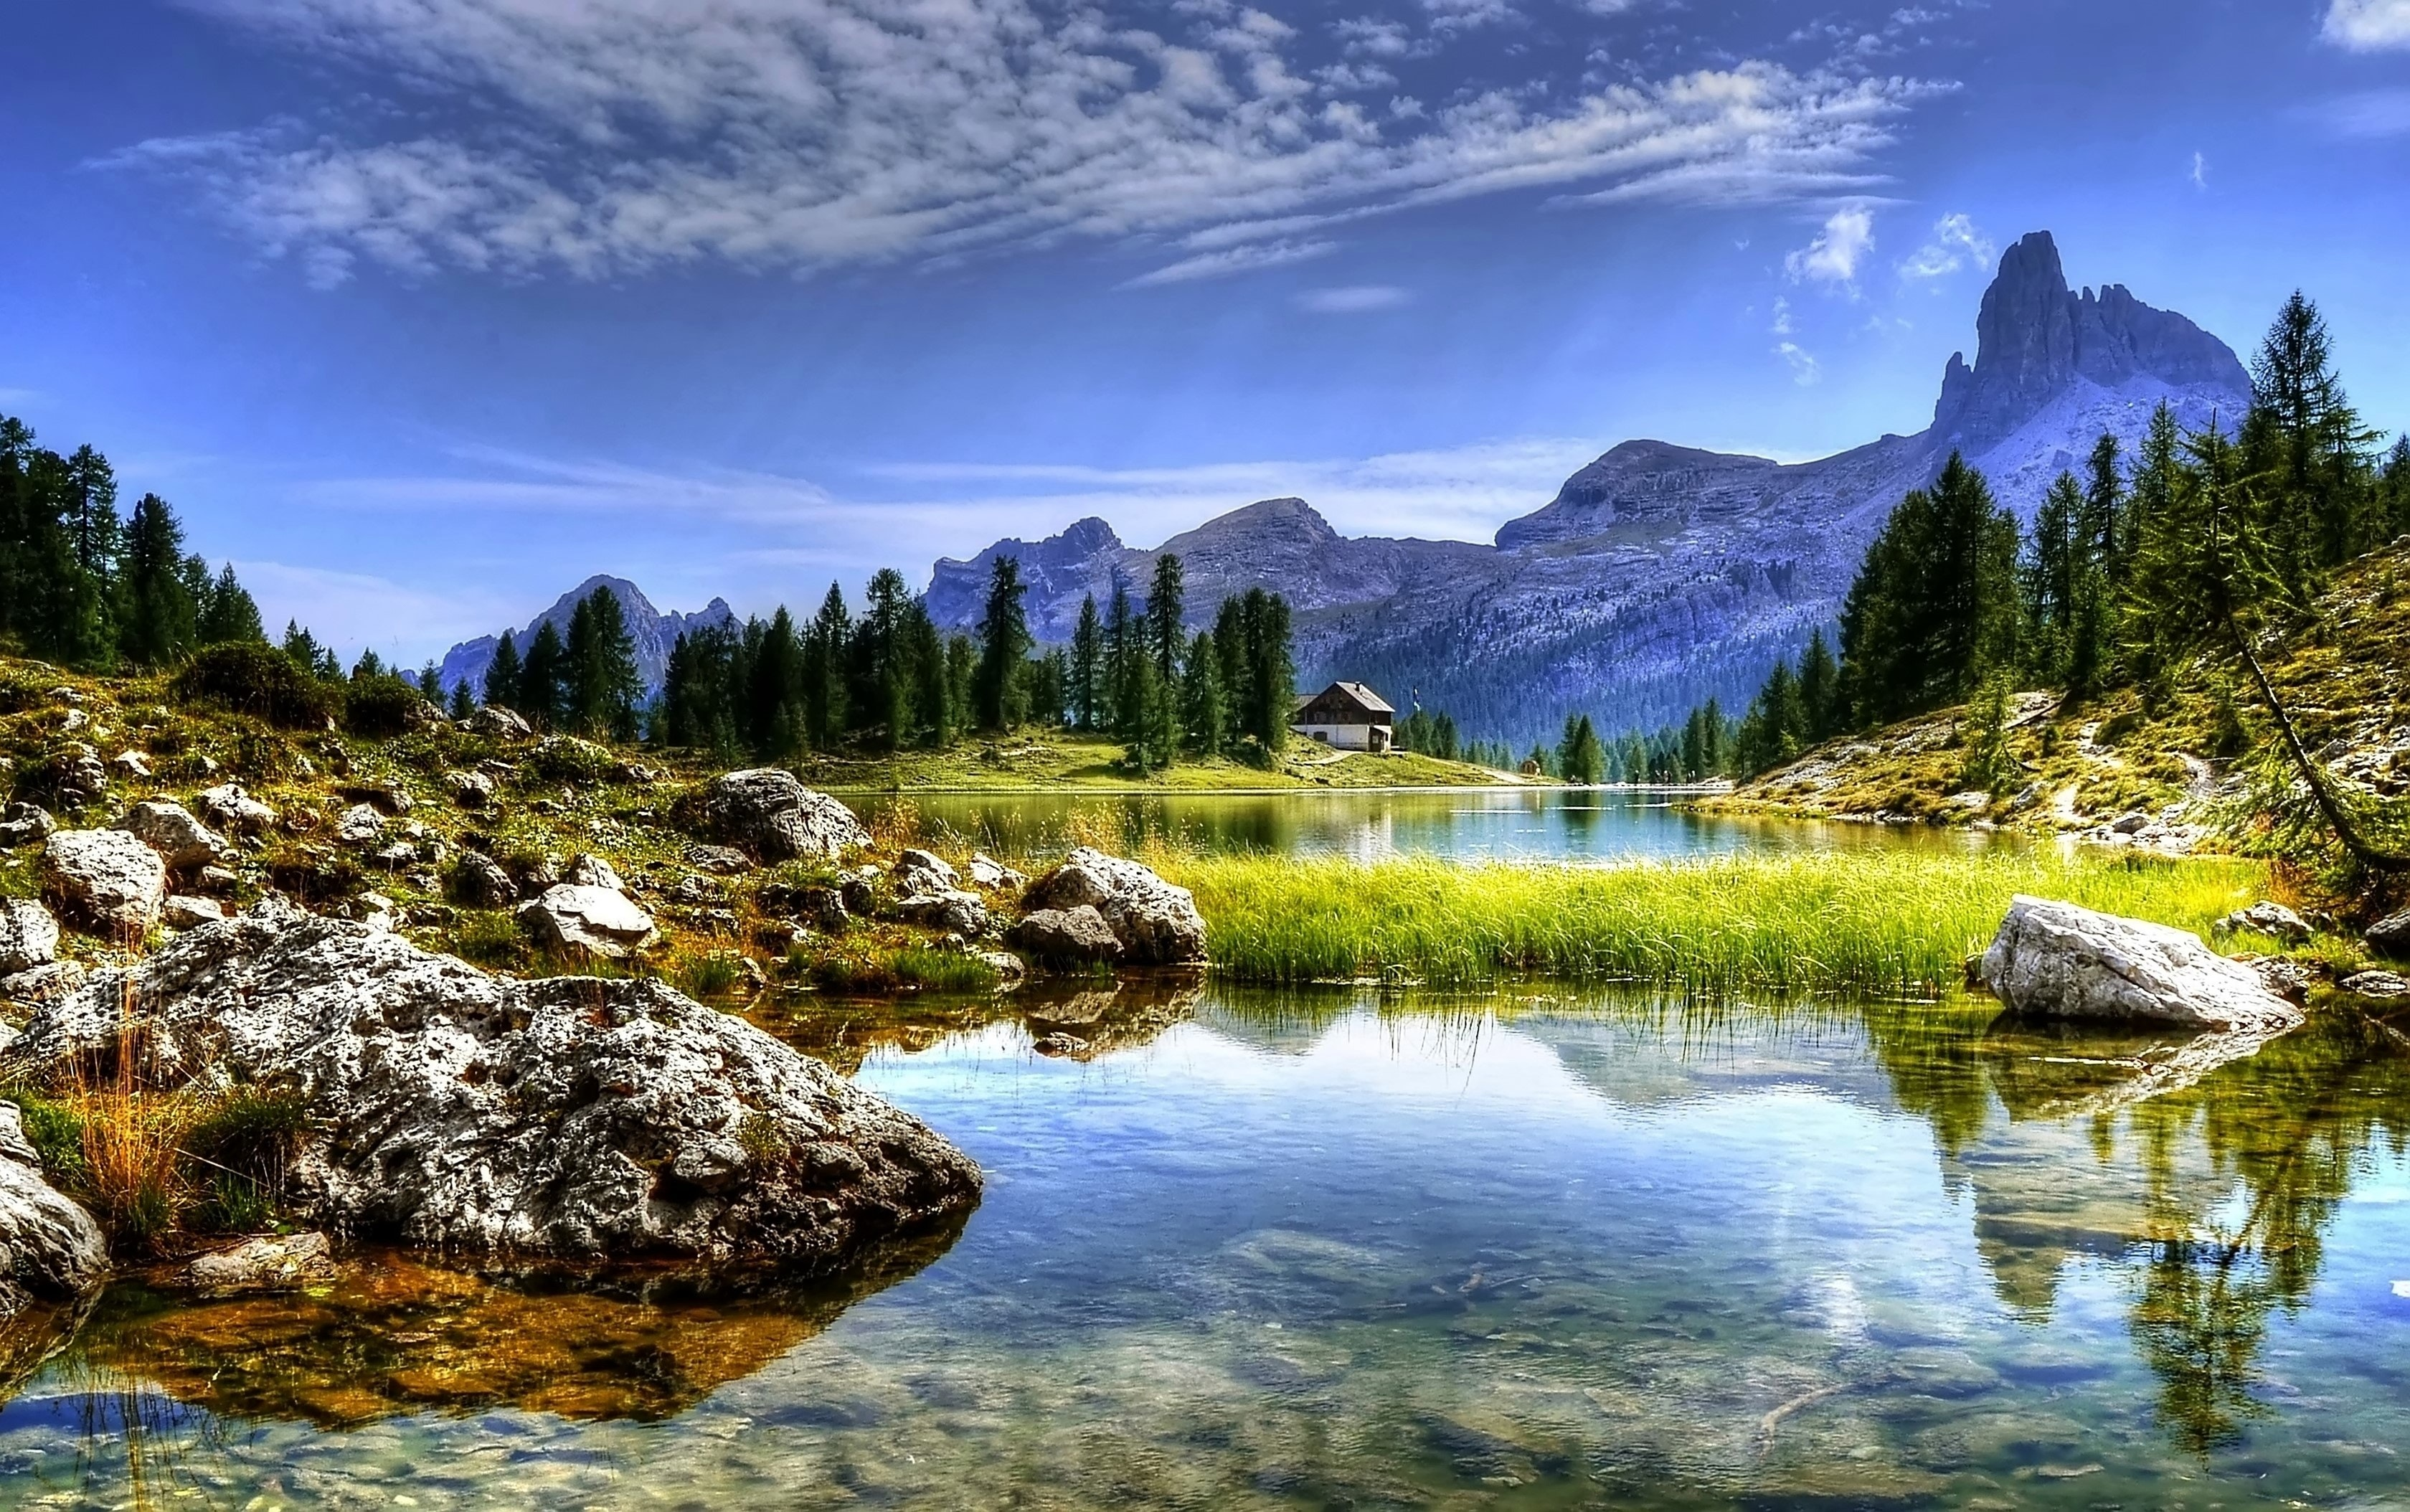
\includegraphics[width=1\textwidth]{images/country.jpg}
\caption{Slika pokrajine, veliko podrobnosti.}
\label{slika2}
\end{center}
\end{figure}

\begin{figure}[htbp]
\begin{center}
\includegraphics[width=1\textwidth]{images/gray.jpeg}
\caption{Sivinska slika.}
\label{slika3}
\end{center}
\end{figure}

\begin{figure}[htbp]
\begin{center}
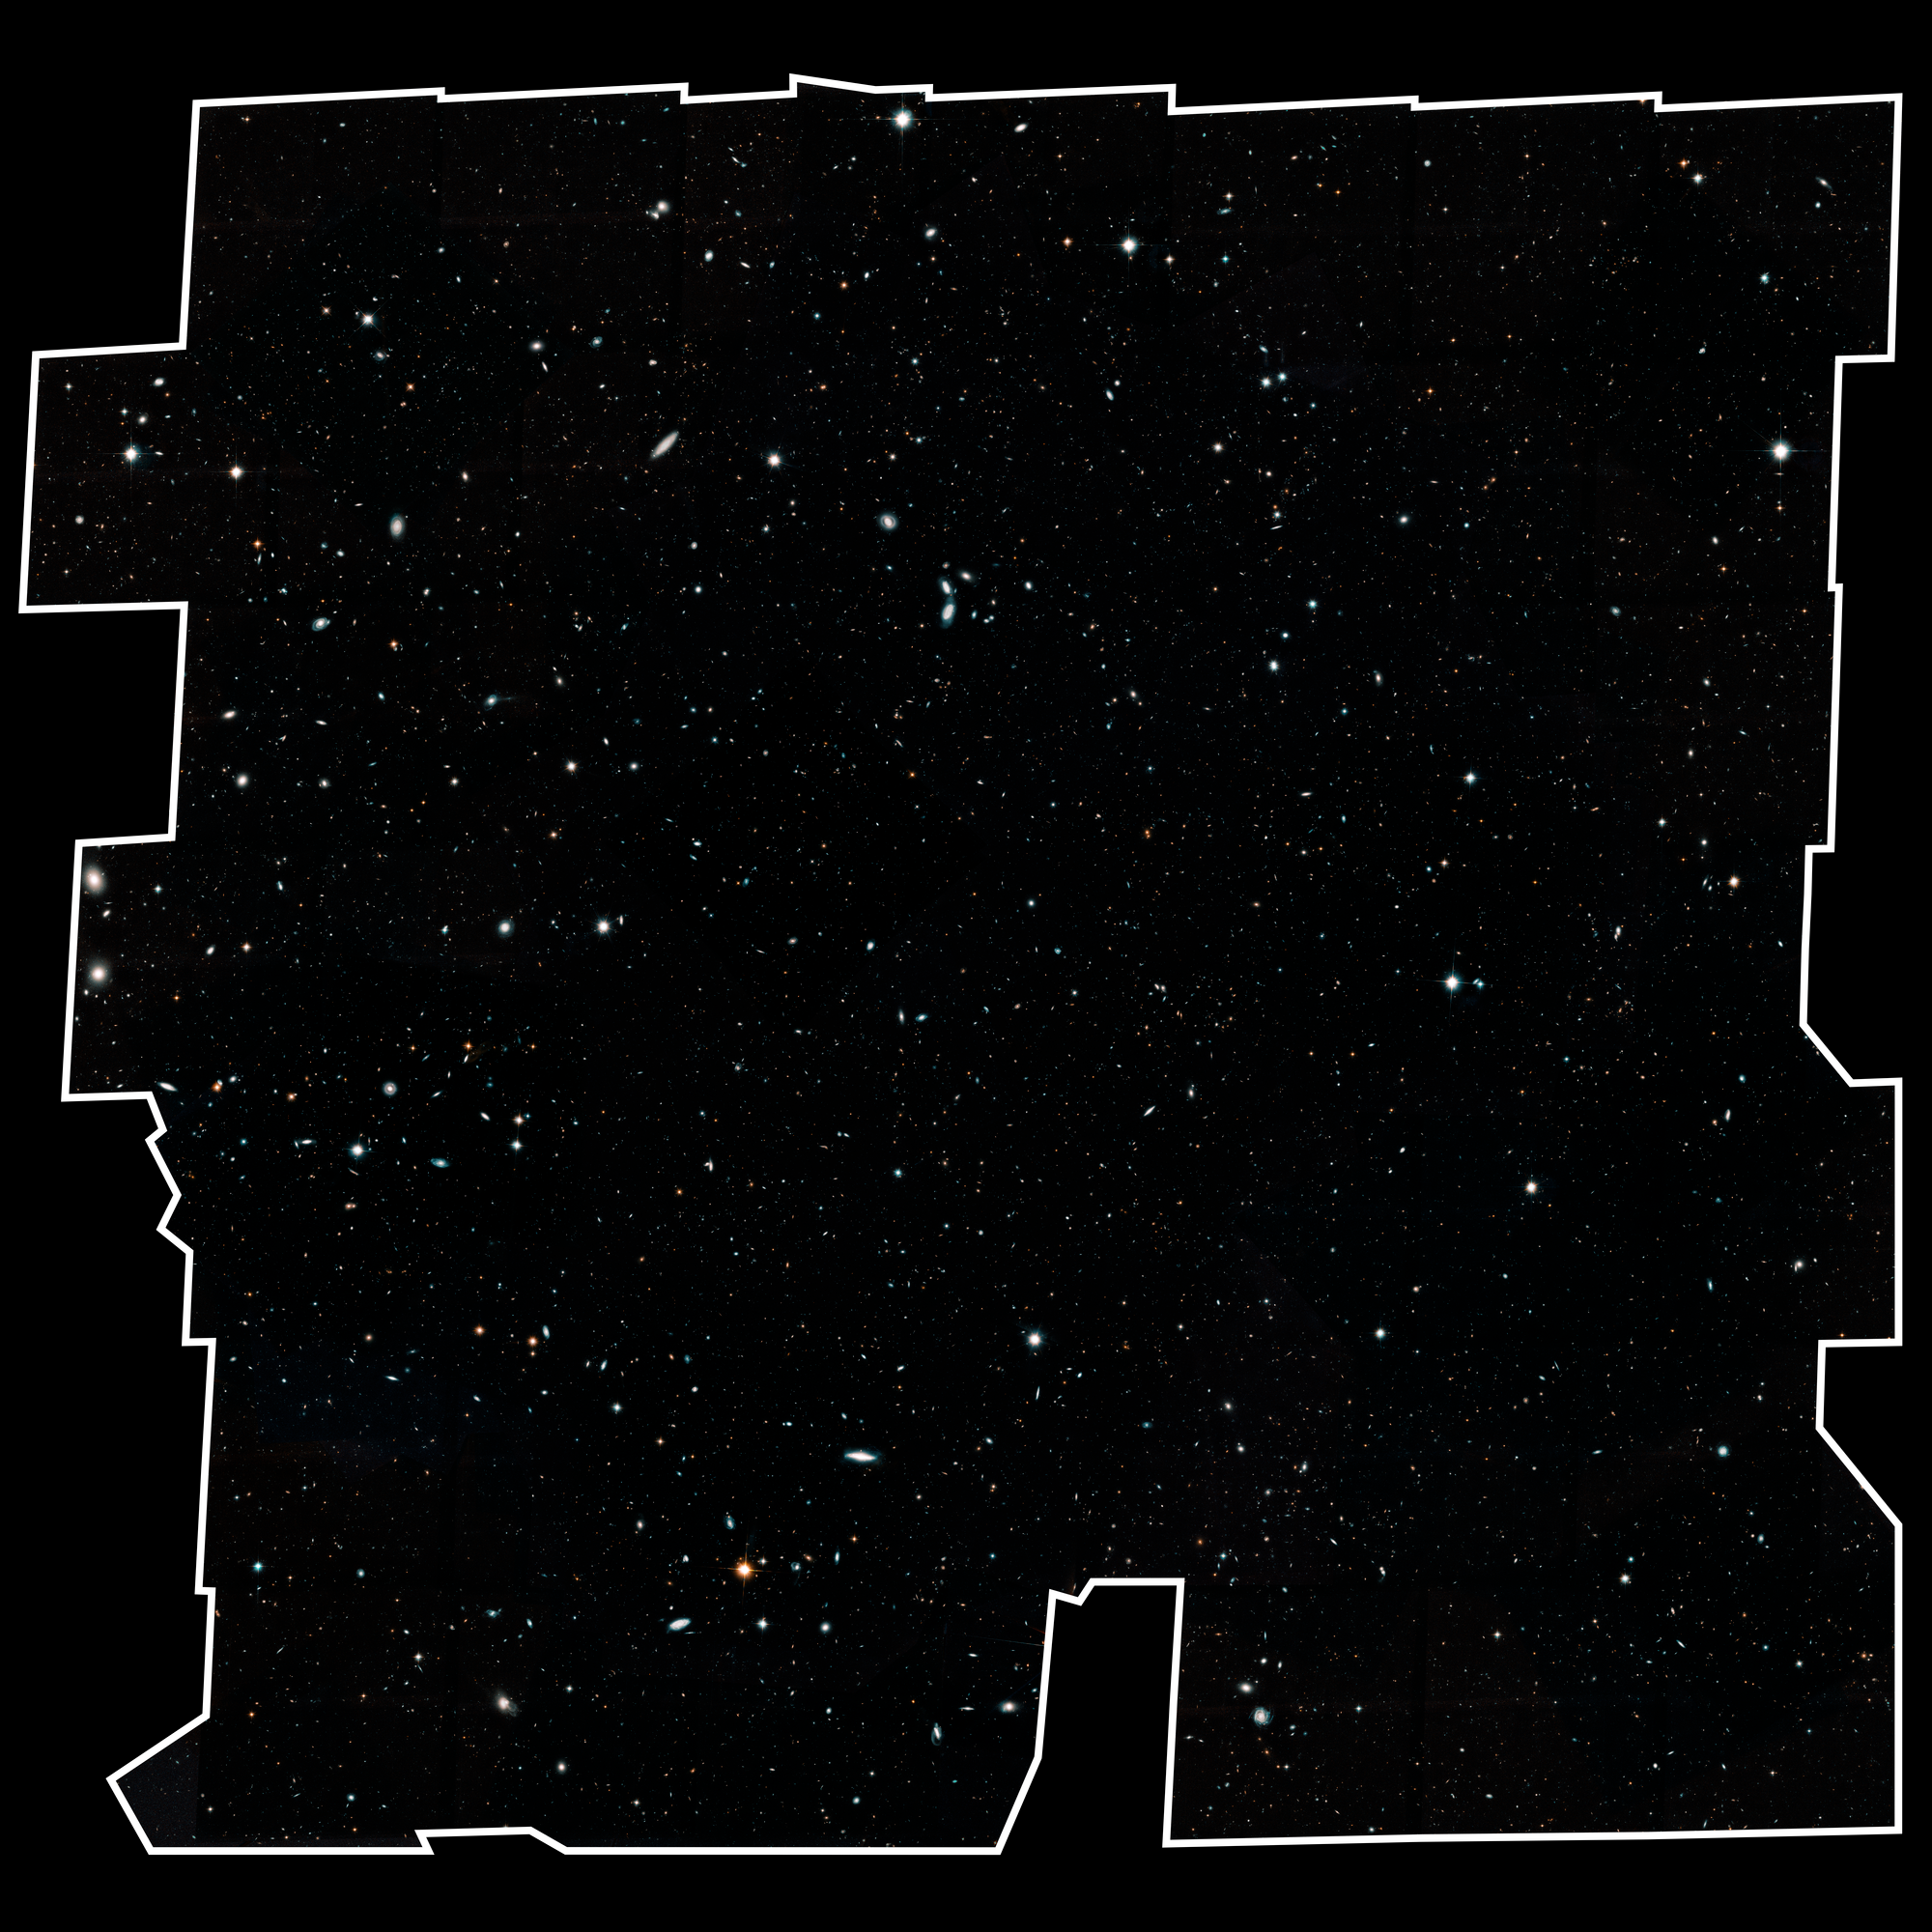
\includegraphics[width=1\textwidth]{images/hubble2000x2000.png}
\caption{Slika vesolja (Hubble), pomembno je ohraniti majhne zvezde.}
\label{slika4}
\end{center}
\end{figure}


\begin{figure}[htbp]
\begin{center}
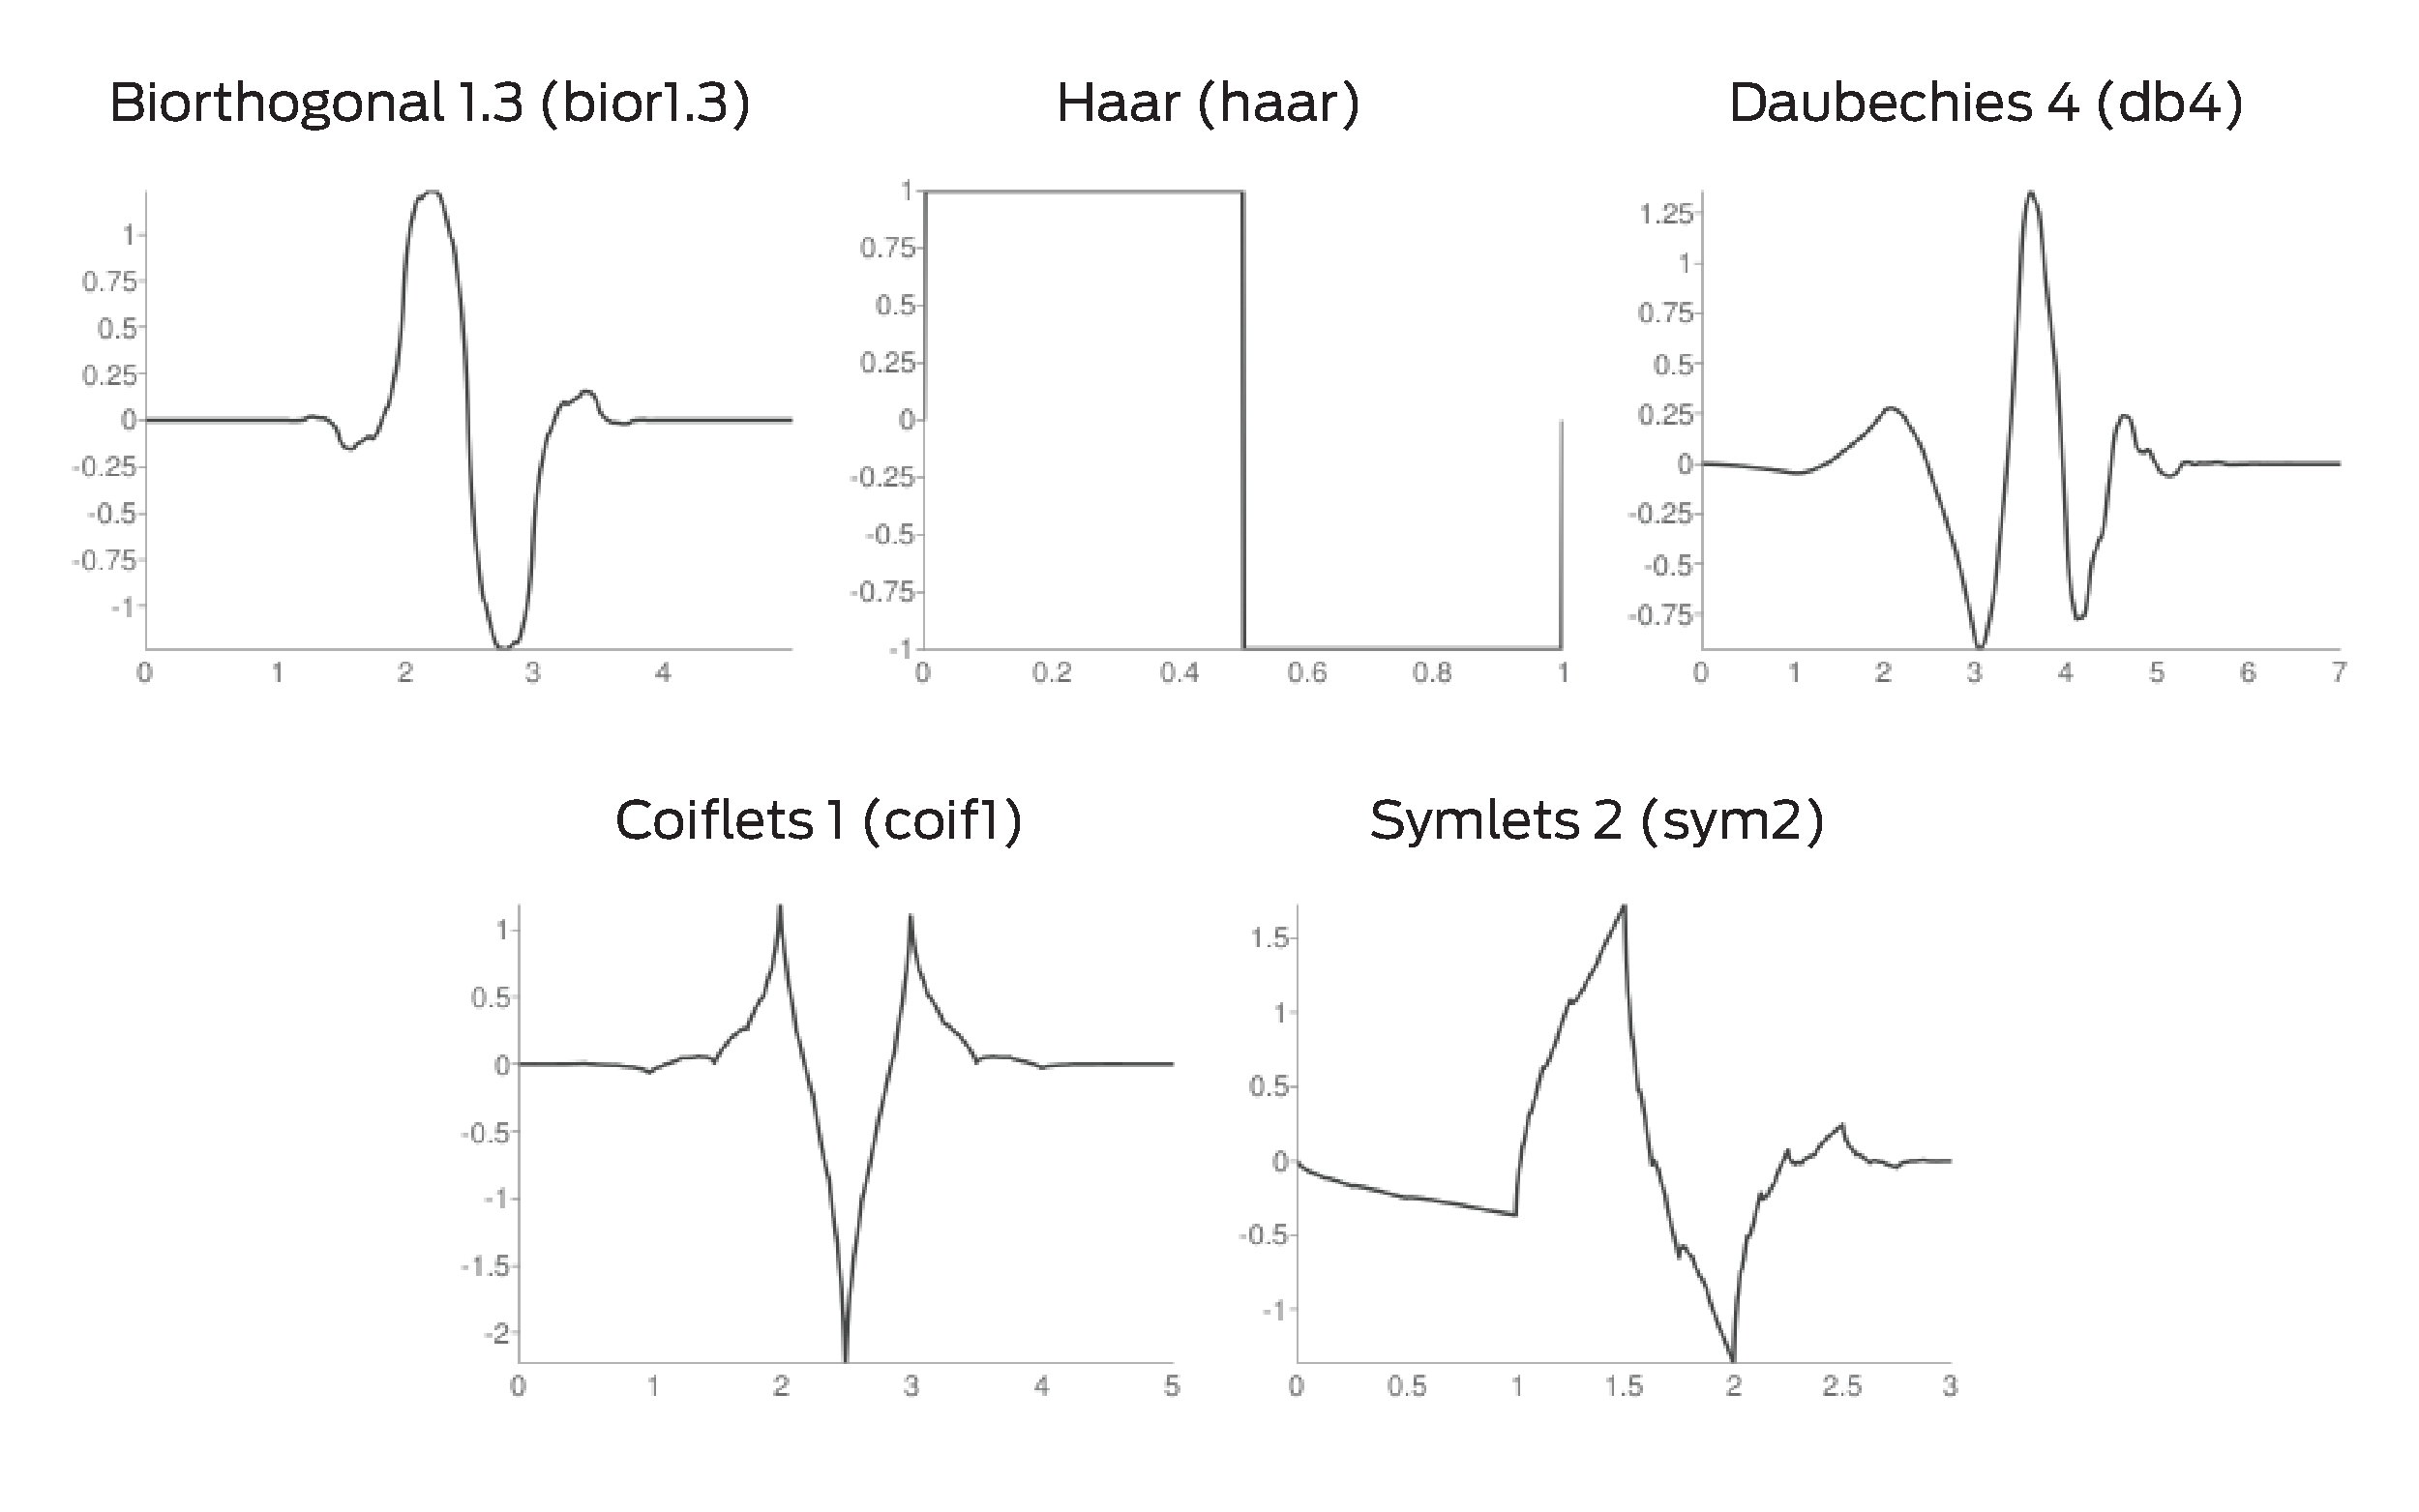
\includegraphics[width=1\textwidth]{images/report/wavelets.pdf}
\caption{Valčki uporabljeni pri testiranju}
\label{wavelets}
\end{center}
\end{figure}

\end{document}
